%----------------------------------------------------------------------------
\section{Monitor forráskód generátor}
%----------------------------------------------------------------------------

%----------------------------------------------------------------------------
\subsection{A monitor interfészei}
%----------------------------------------------------------------------------

A monitorozás alatt lévő rendszer egy közös interfészen keresztül kommunikál a monitorral.
Az interfész \textit{Java} implementációja a 5.5. kódrészleten tekinthető meg.
A monitor azt vizsgálja, hogy a rendszer a scenario szerint működik-e.

Monitor interfész:
\begin{itemize}
    \item \textit{update()}: a monitorban tárolt rendszer állapotát frissíti a paraméterben kapott üzenet alapján.
    \item \textit{goodStateReached()}: a rendszer aktuális állapotát jelzi.
    \item \textit{requirementSatisfied()}: jelzi hogy a rendszer megfelel-e a követelménynek.
    \item \textit{errorDetected()}: detektált hiba jelzésére szolgál.
    \item \textit{noMoreMessages()}: a rendszer jelezheti a kommunikáció végét.
\end{itemize}

Az \textit{update()} függvényt a rendszer hívja, hogy továbbítsa az üzenetet a monitornak.
Paraméterként az üzenet küldőjét (sender), fogadóját (receiver), üzenet nevét (messageType) és az üzenet paramétereit várja (parameters).
A \textit{goodStateReached()} függvény jelzi, hogy a rendszer jelenlegi működése megfelel-e a követelménynek.
A \textit{requirementSatisfied()} függvény visszaadja, hogy a követelmény teljesült-e.
Ha a követelménynek megfelelt a rendszer viselkedése akkor igazat ad vissza, amúgy hamisat.

Az üzenetek megfigyeléséhez szükséges segédfüggvényeket a kommunikációs infrastruktúrához kézzel kell megírni.
Ezek a monitort az \textit{update()} függvényen keresztül hívják.

\begin{lstlisting}[language=java,frame=single, float=h!, caption={Monitor interfész Java implementációja.},captionpos=b]
public interface IMonitor {
	public boolean goodStateReached();
	public void update(String sender, String receiver, String messageType, Map<String, Object> parameters);
	public boolean requirementSatisfied();
	public void errorDetected(String sender, String receiver, String messageType, Map<String, Object> parameters);
	public void noMoreMessages();
}
\end{lstlisting}

Az időzitő komponenshez tartozik egy időzitő interfész amin keresztül elérhető a komponens.
Ezen az interfészen keresztül lehet az óraváltozokat lekérdezni vagy nullázni.
Két függvénye van:

\begin{itemize}
    \item \textit{getClock(String clock)}: óraváltozó lekérdezése név alapján.
    \item \textit{resetClock(String clock)}: óraváltozó nullázása név alapján.
\end{itemize}

\begin{lstlisting}[language=java,frame=single, float=h!, caption={Időzitő interfész Java implementációja.},captionpos=b]
public interface IClock {
	public long getClock(String clock);
	public void resetClock(String clock);
}
\end{lstlisting}

A 5.6. kódrészlet tartalmazza a \textit{IClock} java interfészt.

A monitor az \textit{ISystem} interfészen keresztül tud a rendszernek üzeneteket küldeni a megfigyelt viselkedésről.
Három függvénye van:

\begin{itemize}
	\item \textit{receiveMonitorStatus()}: a monitor jelzi a rendszer felé a követelmény alapján az aktuális státuszt.
	\item \textit{receiveMonitorError()}: a monitor jelzi a rendszer felé ha hibát detektált.
	\item \textit{receiveMonitorSuccess()}: a monitor jelzi a rendszer felé ha teljesült a követelmény.
\end{itemize}

\begin{lstlisting}[language=java,frame=single, float=h!, caption={Rendszer interfész Java implementációja.},captionpos=b]
public interface ISystem {
	public void receiveMonitorStatus(String message);
	public void receiveMonitorError(String actualMessage, String lastAcceptedMessage);
	public void receiveMonitorSuccess();
}
\end{lstlisting}

Az 5.7-es kódrészlet tartalmazza az \textit{ISystem} java interfészt.

%----------------------------------------------------------------------------
\subsection{A monitor forráskód megvalósítása}
%----------------------------------------------------------------------------
A generált forráskód struktúrája egy statikus és egy generált dinamikus részből áll.
A statikus részbe az időzitett automata java osztályai kerülnek:
\begin{itemize}
    \item State: egy állapotot leíró osztály
    \item Transition: egy élet reprezentáló osztály
    \item Automaton: egy automatát megvalósitó osztály
\end{itemize}
A statikus rész a \textit{hu.bme.mit.dipterv.text.util} csomagban található meg, amely a 5.3-as ábrán látható.

A monitor interfész, a monitor Java osztálya, az időzítő interfész és a hozzá tartozó java osztály is ebbe a részbe tartozik.

A dinamikus részben található a \textit{Specification} Java osztály, ami a scenario alapján generált automata forráskódját tartalmazza.

\begin{figure}[!ht]
    \centering
    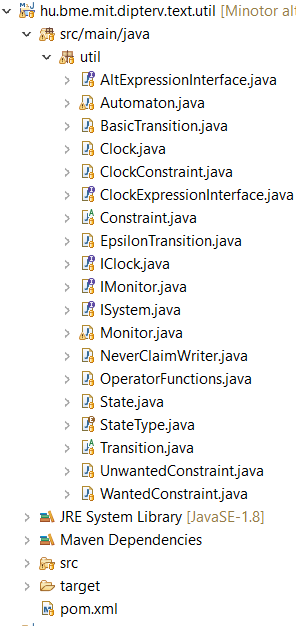
\includegraphics[width=150mm, height= 9cm, keepaspectratio]{figures/util_csomag.png}
    \caption{Az util csomag tartalma.}
\end{figure}

A szükséges forráskódok generálásához az Xtend technológiát használtam.

%----------------------------------------------------------------------------
\clearpage\subsection{Mintapélda}
%----------------------------------------------------------------------------

A 8.3. kódrészleten látható egy scenario követelmény, amit egy okos telefon működésére specifikáltunk.
Az okos telefonon van egy zene lejátszási lista generáló alkalmazás.
A követelményben azt várjuk el, hogy ha a felhasználó megnyitja az alkalmazást akkor a belső kamera készít az arcáról egy képet.
A kép alapján eldönti, hogy milyen a felhasználó kedve és az alapján előállít egy zene lejátszási listát.

A 8.5. kódrészleten látható az okos telefon és a monitor közti kapcsolat megvalósítása Java kódban.
A monitor a rendszertől kapott üzenetek alapján jelzi, hogy a követelmény alapján mi a rendszer állapota.

\begin{lstlisting}[frame=single, float=ht!, caption={Okos telefon működésére megadott scenario követelmény.},captionpos=b]
specification Photo{

	object User user;
	object Device device;
	object Database db;

	constraint error {
		message closeApp() user -> device;
	}

	scenario playlist_generation{
		message openApp() user -> device;
		message accessWebcam() device -> device;
		required message getPhoto() device -> user;
		fail message cameraOffline() user -> device;
		required strict message retrieveMood() device -> db;
		required message retrieveMusic() device -> db;
		strict message generatePlaylist() db -> device;
	}
}
\end{lstlisting}

\begin{lstlisting}[frame=single, float=ht!, caption={Generált automata Never claim formátumba.},captionpos=b]
never{ /*playlist_generationMonitor*/
T0_init:
 if
 :: (!(user.openApp().device)) -> goto T0_init
 :: (user.openApp().device) -> goto T0_q1
 fi;
T0_q1:
 if
 :: (!(device.accessWebcam().device)) -> goto T0_q1
 :: (device.accessWebcam().device) -> goto T0_q2
 fi;
T0_q2:
 if
 :: (!(device.getPhoto().user)) -> goto T0_q2
 :: (!(device.getPhoto().user)) -> goto accept_q3
 :: (device.getPhoto().user) -> goto T0_q4
 fi;
accept_q3:
 if
 fi;
T0_q4:
 if
 :: (!(user.cameraOffline().device)) -> goto T0_q6
 :: (!(user.cameraOffline().device)) -> goto T0_q4
 :: (user.cameraOffline().device) -> goto accept_q5
 fi;
accept_q5:
 if
 fi;
T0_q6:
 if
 :: (device.retrieveMood().db) -> goto T0_q8
 :: (!(device.retrieveMood().db)) -> goto accept_q7
 fi;
accept_q7:
 if
 fi;
T0_q8:
 if
 :: (!(device.retrieveMusic().db)) -> goto T0_q8
 :: (!(device.retrieveMusic().db)) -> goto accept_q9
 :: (device.retrieveMusic().db) -> goto T0_q10
 fi;
accept_q9:
 if
 fi;
T0_q10:
 if
 :: (db.generatePlaylist().device) -> goto T0_q11
 fi;
T0_q11:
 if
 fi;
}
\end{lstlisting}

\begin{lstlisting}[language=java, frame=single, float=ht!, caption={Az okos telefon és hozzá tartozó monitor fel konfigurálásának Java implementációja.},captionpos=b]
public class Main {
	public static void monitorStatus(String status) {
		System.out.println(status);
	}

	public static void main(String[] args) {
		Specification specification = new Specification();
		specification.listAutomatas();
		IMonitor monitor = new Monitor(specification.getAutomata().get(0));

		User user = new User();
		Device device = new Device();
		Database db = new Database();
		user.device = device;
		device.user = user;
		device.db = db;
		db.device = device;
		user.monitor = monitor;
		device.monitor = monitor;
		db.monitor = monitor;

		user.init();
	}
}
\end{lstlisting}

\begin{lstlisting}[language=java, frame=single, float=ht!, caption={Az okos telefon Java osztálya.},captionpos=b]
public class Device {
	public IMonitor monitor;
	public User user;
	public Database db;

	void openApp() {
		monitor.update("user", "device", "openApp", new String[] {});
		accessWebcam();
	}

	void accessWebcam() {
		monitor.update("device", "device", "accessWebcam", new String[] {});
		user.getPhoto();
		db.retrieveMood();
		db.retrieveMusic();
	}

	void cameraOffline() {
		monitor.update("user", "device", "cameOffline", new String[] {});
	}

	void generatePlaylist() {
		monitor.update("db", "device", "generatePlaylist", new String[] {});
	}
}
\end{lstlisting}

A 8.6. kódrészlet az okos telefon Java osztálya.
Megtekinthető a monitor és az eszköz közti kommunikáció megvalósítása is.

\begin{lstlisting}[language=java, frame=single, float=ht!, caption={Monitor kimenete a rendszer működésének egyes fázisaiban.},captionpos=b]
transition: user.openApp().device
q1
System is in bad state.
transition: device.accessWebcam().device
q2
System is in bad state.
transition: device.getPhoto().user
q4
System is in bad state.
transition: !(user.cameraOffline().device)
q6
System is in bad state.
transition: device.retrieveMood().db
q8
System is in bad state.
transition: device.retrieveMusic().db
q10
System is in bad state.
transition: db.generatePlaylist().device
q11
System is in good state.
\end{lstlisting}

A 8.7. kódrészleten látszik, hogy a rendszer a működése elején nem felelt meg a monitor követelményének.
Amikor a működése végére ért akkor a monitor jelezte, hogy a követelmény teljesült a „Good state” üzenettel.
A mintához tartozó Specification osztály a függelékben található.
A generált automatát a konstruktorában állítja elő.

%----------------------------------------------------------------------------
\subsection{Összetett szerkezetek}
%----------------------------------------------------------------------------

A monitor forráskód generátor támogatja az alt, par vagy loop operátorokat tartalmazó scenariokat is.
Erre példát a függelékben lehet találni.

%----------------------------------------------------------------------------
\clearpage\subsection{Időzítési feltételek}
%----------------------------------------------------------------------------

A monitor forráskód generátor támogatja az időzítési feltételeket tartalmazó scenariokat is.
A 8.8. kódrészletben található scenario első üzenetén a "reset x" címke jelzi a monitornak, hogy az "x" óraváltozó nullázni kell.
Egy óraváltozó felvételét is a "reset" címkével lehet végrehajtani.
A 8.9. kódrészlet a példához tartozó Main java osztály leírását tartalmaza, a 8.10. kódrészlet pedig a rendszerhez tartozó Computer java osztályt.
A 8.11. kódrészleten megtekinthető a monitor kimenete.
A kimenet végén lévő "System is in good state." üzenet jelzi, hogy a rendszer működése megfelelt a követeménynek.
A kimenetben szereplő "bad state" üzenetek megtévesztőek lehetnek.
A dolgozat 4. fejezetében említettem, hogy milyen esetekben helyes vagy helytelen a monitor szempontjából a rendszer viselkedése.
A "bad state" üzenet nem feltétlen jelenti azt, hogy a rendszer viselkedése helytelen csupán azt, hogy a feltétel még nem teljesült.
A monitor tovább szeretném fejleszteni a diplomaterv során, úgy hogy pontosabban jelezze a rendszer működésének állapotát.

\begin{lstlisting}[language=java, frame=single, float=ht!, caption={Időzítési feltételeket tartalmazó scenario.},captionpos=b]
specification Email {

	object Computer computer;
	object Server server;

	clock x;

	constraint constraints{
		message logout() computer -> server;
	}

	constraint c {
		message login() server -> computer;
	}

	scenario sendEmail{
		message checkEmail() computer -> computer reset x;
		message sendUnsentEmail() required computer -> server;
		message newEmail() computer -> server pastConstraint {constraints};
		message downloadEmail() computer -> server clockConstraint {x < 10};
	}
}
\end{lstlisting}

\begin{lstlisting}[language=java, frame=single, float=ht!, caption={Időzítéses példához tartozó Main osztály.},captionpos=b]
public class Main {
	public static void monitorStatus(String status) {
		System.out.println(status);
	}

	public static void main(String[] args) {
		Specification specification = new Specification();
		specification.listAutomatas();
		IClock clock = new Clock();
		IMonitor monitor = new Monitor(specification.getAutomata().get(0), clock);

		Server server = new Server(monitor);
		Computer computer = new Computer(server, monitor);
	}
}
\end{lstlisting}

\begin{lstlisting}[language=java, frame=single, float=ht!, caption={A Computer java osztálya.},captionpos=b]
public class Computer {
	public Server server;
	public IMonitor monitor;

	Computer(Server server, IMonitor monitor) {
		this.server = server;
		this.monitor = monitor;
		monitor.update("computer", "computer", "checkEmail", new String[] {});
		checkEmail();
	}

	void checkEmail() {
		monitor.update("computer", "server", "sendUnsentEmail", new String[] {});
		server.sendUnsentEmail();

		monitor.update("computer", "server", "newEmail", new String[] {});
		server.newEmail();

		monitor.update("computer", "server", "downloadEmail", new String[] {});
		server.downloadEmail();
	}
}
\end{lstlisting}

\begin{lstlisting}[language=java, frame=single, float=ht!, caption={Időzítéses példa monitor kimenete.},captionpos=b]
Received Message: computer.checkEmail().computer
Transition: !(computer.checkEmail().computer)
Transition: computer.checkEmail().computer
transition triggered: computer.checkEmail().computer
q1
System is in bad state.
Received Message: computer.sendUnsentEmail().server
Transition: !(computer.sendUnsentEmail().server)
Transition: !(computer.sendUnsentEmail().server)
Transition: computer.sendUnsentEmail().server
transition triggered: computer.sendUnsentEmail().server
q3
System is in bad state.
Received Message: computer.newEmail().server
Transition: !(computer.logout().server) & !(computer.newEmail().server)
Transition: computer.newEmail().server
transition triggered: computer.newEmail().server
q4
System is in bad state.
Received Message: computer.downloadEmail().server
Transition: !(computer.downloadEmail().server)
Transition: computer.downloadEmail().server
transition triggered: computer.downloadEmail().server
q5
System is in good state.
\end{lstlisting}

Az óraváltozók és időzítések megvalósításához az "org.apache.commons.lang3" könyvtár "time" csomag \textit{StopWatch} osztályát használtam.
Ha az automata élén van egy időzítési feltétel akkor a monitor komponens az időzítő komponenstől elkéri a feltételben szereplő óraváltozóban tárol időt és kiértekeli a feltételt.
Ha a feltétel teljesül, akkor az időzítés szempontjából a tranzíció megtörténhet.